\section{Omni XcalableACC Compiler}
We also develop Omni Compiler as a reference implementation for XACC.
Omni Compiler is a source-to-source compiler that translates the base language (C or Fortran) and XACC/XMP directives into runtime calls.

\begin{figure}[!t]
\centering
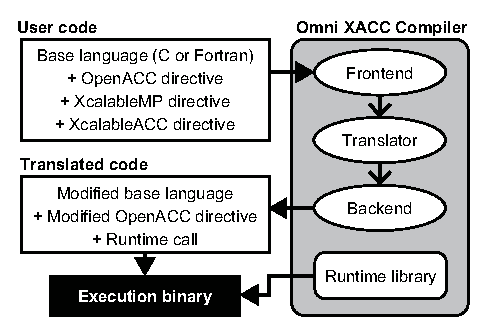
\includegraphics[scale=0.94,clip]{figs/flow2.eps}
\caption{Compile flow of Omni Compiler}
\label{fig:flow}
\end{figure}

Figure \ref{fig:flow} shows the compile flow of Omni Compiler.
First, 
Omni Compiler translates XACC/XMP directives present in the user code into runtime calls. 
Moreover, a part of the base language and OpenACC directives are modified if necessary.
Next, the translated code is compiled by a native compiler to generate an object file.
The native compiler must support OpenACC.
Finally, the object file and the runtime are linked by the native compiler to generate an execution file.
For details on how Omni Compiler translates the user code, please refer to section V of \cite{nakao2014}.

%In order to transfer data between NVIDIA GPUs across compute nodes,
%we implement the following three methods for Omni Compiler.
%(1) Using TCA/IB hybrid communication.
%(2) Using GPUDirect RDMA with CUDA-Aware MPI.
%(3) Using MPI and CUDA.
%Item (1) performs communication with the smallest latency, but a TCA system is required for the computing environment.
%Item (2) is superior in performance to Item (3), but Item (2) also requires specific software and hardware (e.g., MVAPICH2-GDR and Mellanox InfiniBand).
%Whereas Items (1) and (2) can realize direct communication between GPUs without the CPU, 
%Item (3) copies the data from the accelerator memory to the host memory using CUDA and then transfers the data to other compute nodes using MPI.
%Therefore, although Item (3) has the lowest performance, it does not require specific software and hardware.